


\section{Motivation}
\label{sec:motivation}
\begin{figure}[t]
    \centering
        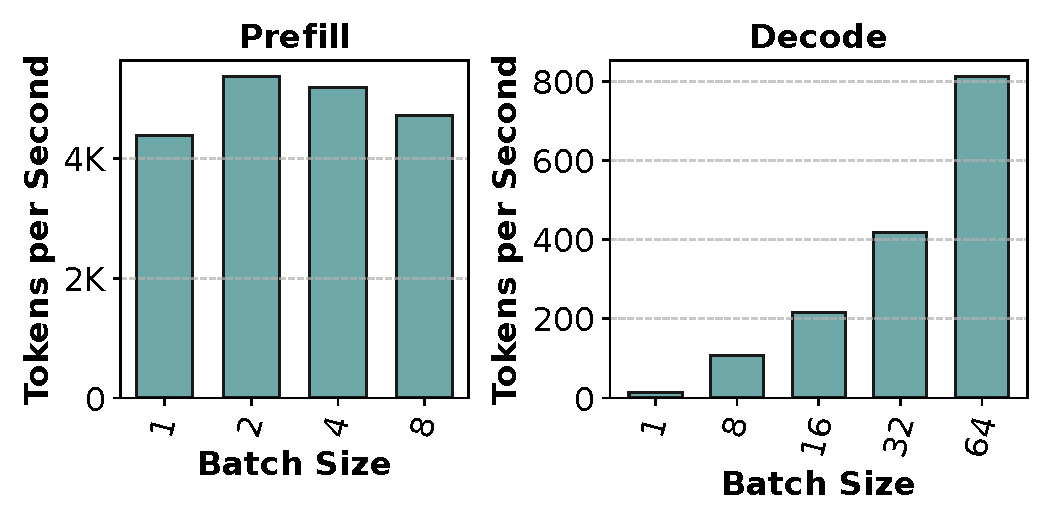
\includegraphics[width=0.47\textwidth]{figures/analysis_tput.pdf}
    \caption{Throughput of the prefill and decode phases with different batch sizes for \mistral running on a single A100 GPU. We use prompt length of 1024 for both prefill and decode experiments. Note that different y-axis, showing prefills are much more efficient than decode. Further, note that \textit{batching boosts decode throughput almost linearly but has a marginal effect on prefill throughput.}}
   \label{fig:background:tput}
\end{figure}


In this section, we first analyse the cost of prefill and decode operations. We then highlight the throughput-latency trade-off and pipeline bubbles that appear in serving LLMs.

\subsection{Cost Analysis of Prefill and Decode}
\label{sec:analysis:throughput}




As discussed in~\autoref{sec:background:inference-process}, while the \textit{prefill} phase processes all input tokens in parallel and effectively saturates GPU compute, the \textit{decode} phase processes only a single token at a time and is very inefficient. \autoref{fig:background:tput} illustrates throughput as a function of batch size, and we can observe that while for decode iterations throughput increases roughly linearly with batch size, prefill throughput almost saturates even with a single request.

\noindent{\bf Takeaway-1:} \textit{The two phases of LLM inference -- prefill and decode -- demonstrate contrasting behaviors wherein batching boosts decode phase throughput immensely but has little effect on prefill throughput.}

\begin{figure}[t]
    \centering
    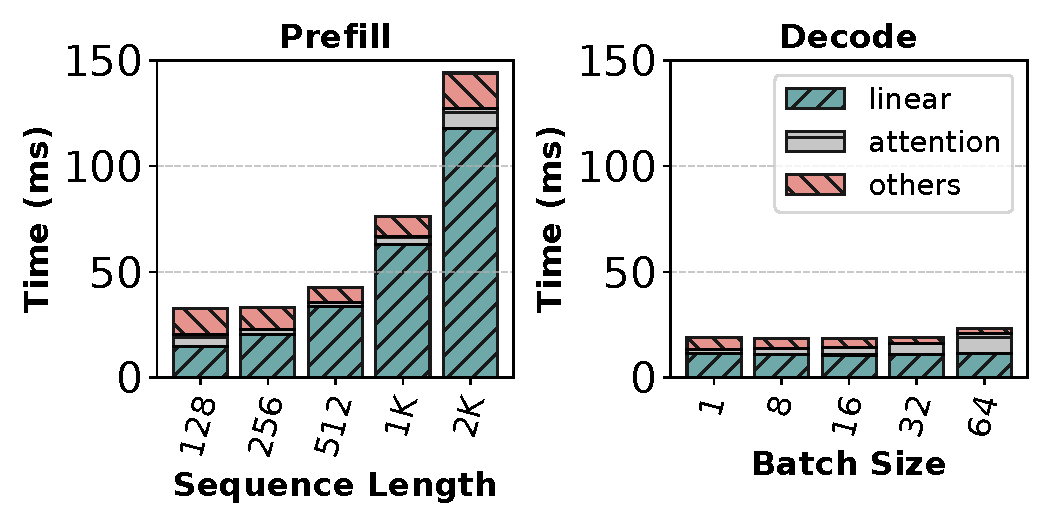
\includegraphics[width=0.47\textwidth]{figures/analysis_pd_breakdown.pdf}
    \caption{Prefill and decode time with different input sizes for \mistral running on single A100 GPU. Linear layers contribute to the majority of runtime in both prefill and decode phases. Due to the low arithmetic intensity in decode batches, the cost of linear operation for 1 decode token is nearly same as 128 prefill tokens. }
    \label{fig:motivation:op-wise-time}
\end{figure}


\if
To illustrate this, we compute the per-token prefill and decode times in \autoref{fig:analysis_per_token} for different input sizes. We vary the model's input size either by varying prompt length using batch size of one (for prefill) or varying batch size (for decode). We can conclude the following from this experiment.


\noindent{\bf Takeaway-1:} \textit{A single prefill request with modest sequence length can effectively saturate GPU compute}. As can be seen in ~\autoref{fig:analysis_per_token}, the prefill throughput increases almost linearly at low sequence lengths, and saturates quickly around sequence length as low as 512 tokens. Thus, even small sequence lengths can provide enough parallelism in the prefill phase to use the GPU compute effectively. This motivates the use of \chunking in \sysname.



Note that for very long sequence lengths \eg 16K, per-token prefill time increases slightly. This is due to the cost of attention operator which grows quadratically with sequence length.

The saturation point depends the model's hidden size and deployment configuration. For example, models with higher embedding size will saturate prefill throughput at smaller sequence lengths while models deployed with large degree of tensor-parallelism will require more tokens to saturate since the amount of computation per-GPU becomes smaller.

\begin{figure}[t]
    \centering
    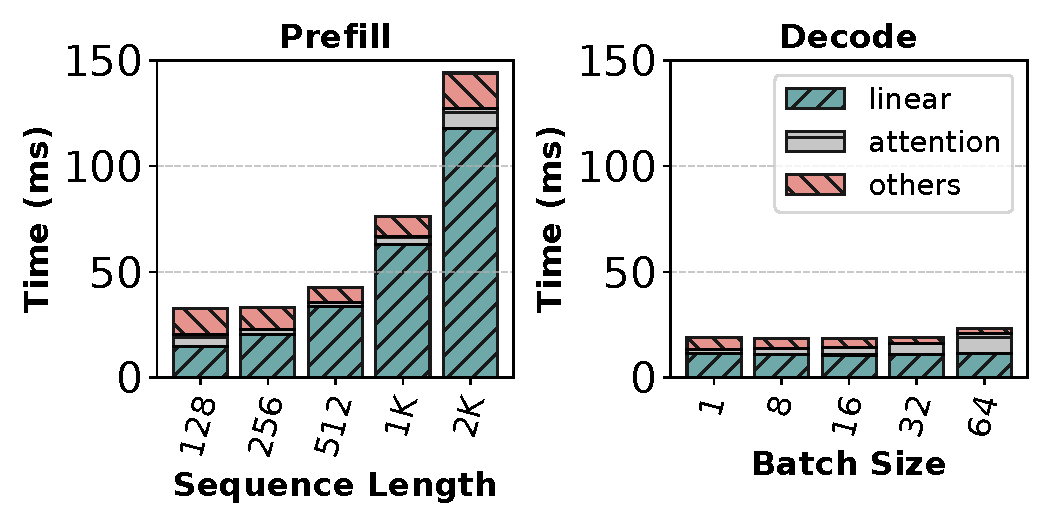
\includegraphics[width=0.47\textwidth]{figures/analysis_pd_breakdown.pdf}
    \caption{Prefill and decode time with different input sizes for \mistral running on single A100 GPU. Linear layers contribute to the majority of runtime in both prefill and decode phases. Due to the low arithmetic intensity in decode batches, the cost of linear operation for 1 decode token is nearly same as 128 prefill tokens. }
    \label{fig:motivation:op-wise-time}
\end{figure}

\noindent{\bf Takeaway-2:} \textit{The decode time per token is order(s) of magnitude higher than prefill, especially at small batch sizes}. As shown in ~\autoref{fig:analysis_per_token}, at a very high decode batch size of 128, the per-token decode time is still $4.4\times$ higher than the lowest prefill time per-token. Note that the decode time per token improves almost linearly with batch size. At 16, which is in lower side of decode batch sizes, the per-token decode time is still 20X. Thus, optimizing decodes is crucial for efficient LLM inference.
\fi

\autoref{fig:motivation:op-wise-time} breaks down the prefill and decode compute times into linear, attention and others, and shows their individual contributions. From the figure, we see that linear operators contribute to the majority of the runtime cost.  While attention cost grows quadratically with sequence length, linear operators still contribute more than 80\% to the total time even at high sequence lengths. Therefore, optimizing linear operators is important for improving LLM inference.



\noindent{\bf Low Compute Utilization during Decodes:} Low compute utilization during the decode phase is a waste of GPU's processing capacity. To understand this further, we analyze the arithmetic intensity of prefill and decode iterations. Since the majority of the time in LLM inference is spent in linear operators, we focus our analysis on them.





Matrix multiplication kernels overlap memory accesses along with computation of math operations. The total execution time of an operation can be approximated to $T = \text{max}(T_{\text{math}}, T_{\text{mem}})$, where $T_{\text{math}}$ and $T_{\text{mem}}$ represent the time spent on math and memory fetch operations respectively. An operation is considered memory-bound if $T_{\text{math}} < T_{\text{mem}}$. Memory-bound operations have low Model FLOPs Utilization (MFU) \cite{chowdhery2022Palm}. On the other hand, compute-bound operations have low Model Bandwidth Utilization (MBU).
When $T_{\text{math}} = T_{\text{mem}}$, both compute and memory bandwidth utilization are maximized. Arithmetic intensity quantifies the number of math operations performed per byte of data fetched from the memory. At the optimal point, the arithmetic  intensity of operation matches the FLOPS-to-Bandwidth ratio of the device. \autoref{fig:motivation:arithmatic-intensity} shows arithmetic intensity as a function of the number of tokens in the batch for linear layers in \llamaL running on four A100 GPUs. Prefill batches amortize the cost of fetching weights of the linear operators from HBM memory to GPU cache over a large number of tokens, allowing it to have high arithmetic intensity. In contrast, decode batches have very low computation intensity. \autoref{fig:motivation:mlp-time} shows the total execution time of linear operators in an iteration for \llamaL as a function of the number of tokens. Note that execution time increases only marginally in the beginning \ie as long as the batch is in a memory-bound regime, but linearly afterwards \ie when the batch becomes compute-bound.\footnote{Theoretically, we expect the operators to become compute-bound at $\sim$200 tokens on A100 GPUs, however, in practice we observe that it happens at $\sim$500-600 tokens for higher tensor parallel dimensions due to fixed overheads.}

\begin{figure}[t!]
    \centering
        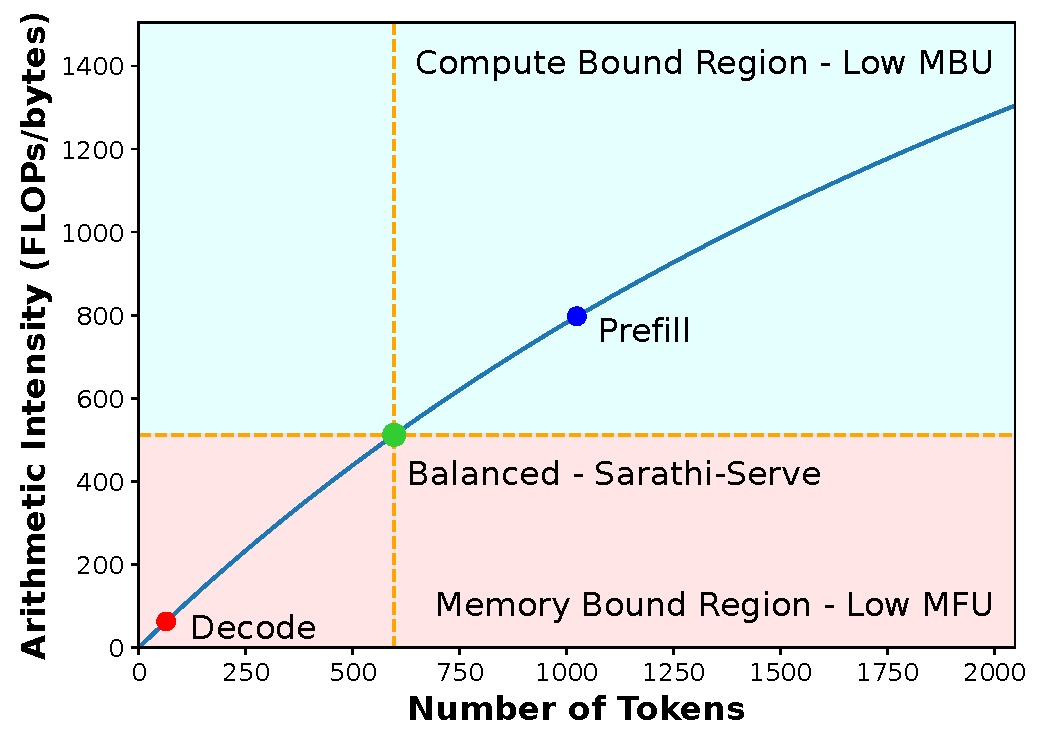
\includegraphics[width=0.45\textwidth]{figures/arithmetic_intensity.pdf}
        
    \caption{Arithmetic intensity trend for \llamaL linear operations with different number of token running on four A100s. Decode batches have low arithmetic intensity \ie they are bottlenecked by memory fetch time, leading to low compute utilization. Prefill batches are compute bound with sub-optimal bandwidth utilization. \sysname forms balanced batches by combining decodes and prefill chunks to maximize both compute and bandwidth utilization.}
       \label{fig:motivation:arithmatic-intensity}
\end{figure}






\noindent{\bf Takeaway-2:} \textit{Decode batches operate in memory-bound regime leaving compute underutilized. This implies that more tokens can be processed along with a decode batch without significantly increasing its latency.} %

\begin{figure}[t!]
    \centering
    \hspace{-12px}
    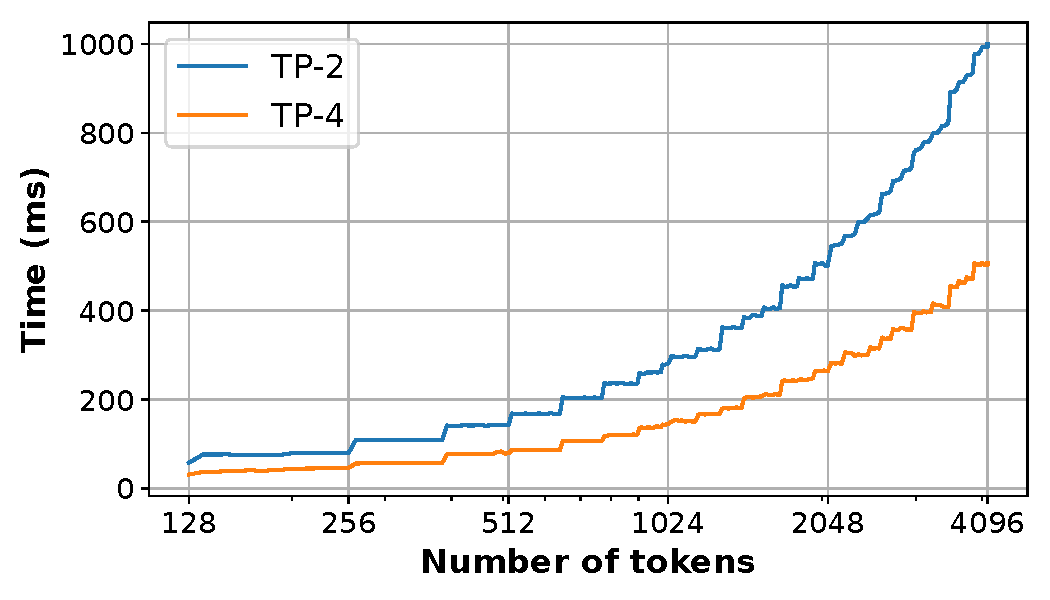
\includegraphics[width=0.45\textwidth]{figures/mlp_num_tokens_vs_time.pdf}
    \caption{Linear layer execution time as function of number of tokens in a batch for \llamaL on A100(s) with different tensor parallel degrees. When the number of tokens is small, execution time is dictated by the cost of fetching weights from HBM memory. Hence, execution time is largely stagnant in the 128-512 tokens range, especially for higher tensor parallel degrees. Once the number of tokens in the batch cross a critical threshold, the operation become compute bound and the runtime increases linearly with number of tokens.}%
    \label{fig:motivation:mlp-time} 
\end{figure}

\begin{figure}[t!]
    \centering
        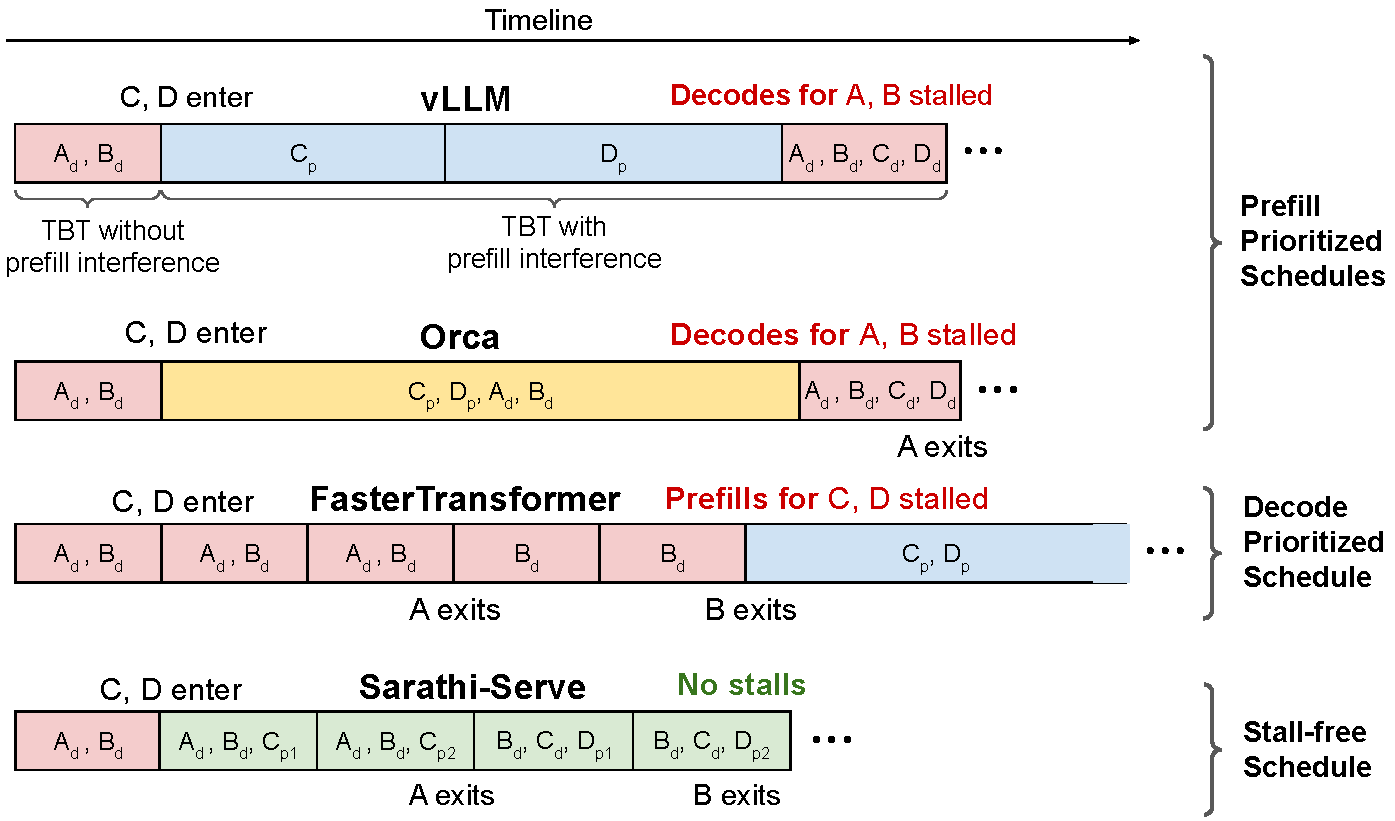
\includegraphics[width=0.47\textwidth]{figures/sarathi_server_timeline.pdf}
    \caption{A generation stall occurs when one or more prefills are scheduled in between consecutive decode iterations of a request. A, B, C and D represent different requests. Subscript $d$ represents a decode iteration, $p$ represents a full prefill and $p0$, $p1$ represent two chunked prefills of a given prompt. vLLM induces generation stalls by scheduling as many prefills as possible before resuming ongoing decodes. Despite supporting hybrid batches, Orca cannot mitigate generation stalls because the execution time of batches containing long prompts remains high. FasterTransformer is free of generation stalls as it finishes all ongoing decodes before scheduling a new prefill but compromises on throughput due to low decode batch size. In contrast, \sysname generates a schedule that eliminates generation stalls yet delivers high throughput.}
        \label{fig:motivation:generationstalls}
\end{figure}

\subsection{Throughput-Latency Trade-off}
\label{sec:latencyandstalls}



\Ils improves system throughput but we show that it comes at the cost of high TBT latency due to a phenomenon we call \textit{generation stalls}.


\autoref{fig:motivation:generationstalls} compares different scheduling policies. The example shows a timeline (left to right) of requests A, B, C and D. Requests A and B are in decode phase at the start of the interval and after one iteration, requests C and D enter the system. Orca and vLLM both use FCFS \ils with eager admission of prefill requests %
but differ in their batch composition policy. Orca supports hybrid batches composed of both prefill and decode requests whereas vLLM only supports batches that contain either all prefill or all decode requests. Irrespective of this difference, both Orca and vLLM can improve throughput by maximizing the batch size in subsequent decode iterations. However, eagerly scheduling prefills of requests C and D delays the decodes of already running requests A and B because an iteration that computes one or more prefills can take several seconds depending on the lengths of input prompts. Therefore, \prefillprio schedulers can introduce \textit{generation stalls} for ongoing decodes resulting in latency spikes caused by high TBT.




In contrast to \ils, \rls systems such as FasterTransformer \cite{fastertransformer} do not schedule new requests until \textit{all} the already running requests complete their decode phase (line 3 in \autoref{alg:request_level}). In \autoref{fig:motivation:generationstalls}, the prefills for requests C and D get stalled until requests A and B both exit the system. Therefore, \decodeprio systems provide low TBT latency albeit at the cost of low system throughput. For example, Kwon et al. \cite{vllmsosp} show that \ils with PagedAttention can achieve an order of magnitude higher throughput compared to FasterTransformer.

One way to reduce latency spikes in \ils systems is to use smaller batch sizes as recommended in Orca~\cite{orca}. However, lowering batch size adversely impacts throughput as shown in~\autoref{sec:background:inference-process}. Therefore, existing systems are forced to trade-off between throughput and latency depending on the desired SLOs.


\noindent{\bf Takeaway-3:} \textit{The interleaving of prefills and decodes involves a trade-off between throughput and latency for current LLM inference schedulers. State-of-the-art systems today use prefill-prioritizing schedules that trade TBT latency for high throughput.}




\begin{figure}[!t]
    \centering
    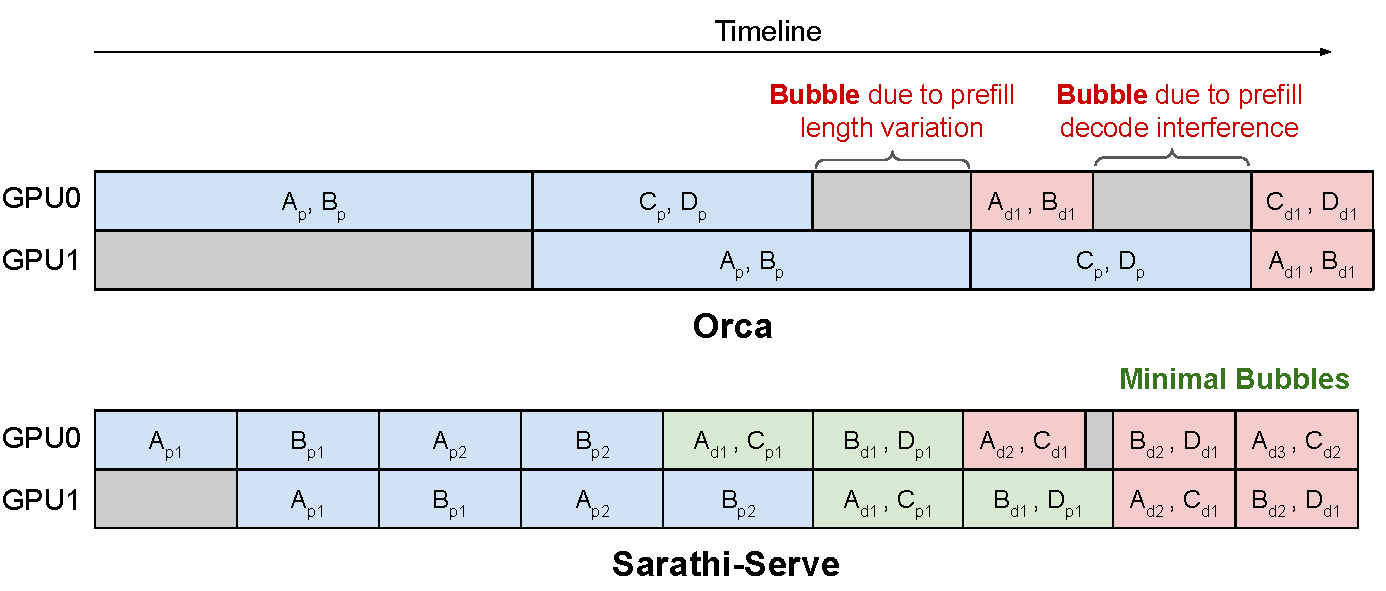
\includegraphics[width=0.43\textwidth]{figures/pp-bubble-new.pdf}
    \caption{A 2-way pipeline parallel iteration-level schedule in Orca across 4 requests (A,B,C,D) shows the existence of pipeline bubbles due to non-uniform batch execution times. \sysname is able to minimize these stalls by creating uniform-compute batches.}
    \label{fig-mot-bubbles}
\end{figure}

\subsection{Pipeline Bubbles waste GPU Cycles}
Pipeline-parallelism (PP) is a popular strategy for cross-node deployment of large models, owing to its lower communication overheads compared to Tensor Parallelism (TP). A challenge with PP, however, is that it introduces \textit{pipeline bubbles} or periods of GPU inactivity as subsequent pipeline stages have to wait for the completion of the corresponding micro-batch in the prior stages. Pipeline bubbles is a known problem in training jobs, where they arise between the forward and backward passes due to prior stages needing to wait for the backward pass to arrive. Micro-batching is a common technique used in PP training jobs to mitigate pipeline bubbles~\cite{varuna,pipedream,gpipe}. 

Inference jobs only require forward computation and therefore one might expect that micro-batching can eliminate pipeline bubbles during inference. In fact, prior work on transformer inference, such as, FasterTransformer~\cite{fastertransformer} and FastServe~\cite{fastserve} use micro-batches but do not mention pipeline-bubbles.  Recently proposed Orca~\cite{orca} also suggests that iteration-level scheduling eliminates bubbles in pipeline scheduling (see Figure 8 in ~\cite{orca}). However, our experiments show that even with iteration-level scheduling, pipeline bubbles can waste significant GPU cycles with PP (\autoref{sec-eval-pp}).



Each micro-batch (or iteration) in LLM inference can require a different amount of compute (and consequently has varying execution time), depending on the composition of prefill and decode tokens in the micro-batch (see~\autoref{fig-mot-bubbles}). We identify three types of bubbles during inference: (1) bubbles like $PB_1$ that occur due to the varying number of prefill tokens in two consecutive micro-batches (2) bubbles like $PB_2$ that occur due to different compute times of prefill and decode stages when one is followed by the other, and (3) bubbles like $PB_3$ that occur due to difference in decode compute times between micro-batches since the attention cost depends on the accumulated context length  (size of the KV-cache) and varies across requests. For Falcon-180B, a single prompt of 4k tokens takes $\approx1150$ ms to execute compared to a decode only iteration with batch size 32 which would take about $\approx200$ ms to execute. Interleaving of these iteration could result in a bubble of $\approx950$ ms. These pipeline bubbles are wasted GPU cycles and directly correspond to a loss in serving throughput and increased latency. This problem is aggravated with increase in prompt lengths and batch size, due to longer and more frequent prefill iterations respectively. If we can ensure that each micro-batch performs uniform computation, we can mitigate these pipeline bubbles.

\noindent{\bf Takeaway-4:} \textit{There can be a large variance in compute time of LLM iterations depending on composition of prefill- and decode-tokens in the batch. This can lead to significant bubbles when using pipeline-parallelism.}

